\chapter{The Software Heritage Graph Dataset}

\section{Introduction}
\label{sec:intro}

Public software development, i.e., the practice of collaboratively developing
software using collaborative development platforms (also known as
``forges''~\cite{DBLP:conf/wikis/Squire17}) such as GitHub or GitLab is now
well established. Further source code distribution mechanisms, by the means of
\textsc{gnu}/Linux distributions and language-specific package
managers~\cite{DBLP:conf/msr/KikasGDP17, DBLP:conf/msr/AbateCGFTZ15} are also
becoming more and more popular, realizing in practice the half-century-old
vision of off-the-shelf software components~\cite{mcilroy1968mass,Spi07a}.

The extensive public availability of software source code artifacts (source code
files, commits, release information, etc.) is a significant asset for mining
software repositories and, more generally, empirical software engineering
research.
The topics of corresponding studies range from the study of code
clones~\cite{SvajlenkoR17, SemuraYCI17, ThummalapentaCAP10} to automated
vulnerability detection and repair~\cite{Li2017, Grieco2016, MartinezM15};
and from
code recommenders~\cite{Zeller2007, ZimmermannWDZ04} to software licence
analysis and license compliance~\cite{GermanLicense17, VendomeLicence2015}.
However, many research studies are still being conducted on
significantly smaller \emph{subsets} of the \emph{entire corpus of publicly
  available source code artifacts}.

The \SWH project~\cite{cacm-2018-software-heritage,
  ipres-2017-software-heritage} aims at fixing this gap, by collecting,
preserving, and sharing the entire body of publicly available software source
code, together with the associated development history, as it is captured by
modern version control systems (\textsc{vcs})~\cite{spinellis2005version}.

In this paper we introduce the \emph{\SWHGD}, a graph representation of all the
source code artifacts archived by \SWH{}. The graph is a fully deduplicated
Merkle \textsc{dag}~\cite{Merkle} that links together: source code file contents, source
trees (directories) containing them, \textsc{vcs} commits and releases, up to crawling
information indicating when and where (\textsc{url}s) a given VCS repository state
(which in turn binds all other artifacts together) has been observed.

% TODO: update figures if we make a new version of the dataset
The dataset captures the state of the \SWH{} archive on September 25th 2018,
spanning a full mirror of Github and GitLab.com, the Debian distribution,
Gitorious, Google Code, and the PyPI repository. Quantitatively it corresponds
to 5 billion unique file contents and 1.1 billion unique commits, harvested
from more than 85 million software origins (see Section~\ref{sec:data-model} for more
detailed figures).


\paragraph*{Dataset availability}

The \SWH{} graph is encoded in the dataset as a set of relational
tables---roughly, one for each node type; see Section~\ref{sec:data-model} for
details---that can be queried using \textsc{SQL}. The dataset is available in three
alternative formats, catering for different use cases:
\begin{itemize}

\item a Postgres~\cite{stonebraker1991postgres} \textbf{database dump} in \textsc{csv}
  format (for the data) and \textsc{ddl} queries (for recreating the DB schema): this
  format is best for local processing on a single server or high-end
  workstation;

\item a set of \textbf{Apache Parquet files}~\cite{website-apache-parquet}
  suitable for loading into columnar storage and scale-out processing
  solutions, e.g., Apache Spark~\cite{zaharia2016apache};

\item a public dataset on \textbf{Amazon Athena}~\cite{website-amazon-athena},
  where the sample queries of Section~\ref{sec:usage} can be tried live.

\end{itemize}

The first two formats are available for download ($\approx$1~TiB each) from
Zenodo at
\url{https://zenodo.org/record/2583978}, (\doi{10.5281/zenodo.2583978}).
The Athena dataset\footnote{\url{https://registry.opendata.aws/software-heritage/}} can also be
queried from the \textsc{AWS} console by following the instructions in the
\texttt{README.md} file.

\begin{comment}

\paragraph*{Paper structure}

In the following we describe the data gathering process used to assemble the
dataset (Section~\ref{sec:gathering}), present the data model
(Section~\ref{sec:data-model}), provide a brief usage tutorial and ideas
for research questions that can be answered using the dataset
(Section~\ref{sec:usage}), discuss dataset limitations and future extensions
(Section~\ref{sec:threats}).

\end{comment}


\section{Data Gathering}
\label{sec:gathering}

The \SWHGD has been assembled as part of the regular crawling activities of
\SWH, dating back to 2015. Due to the long-term archival
nature of \SWH, the dataset is not entirely reproducible, because the archived
source code artifacts might have disappeared from the original hosting place: a
\textsc{vcs} might have been deleted, a commit or branch rewritten (e.g., using
\texttt{git rebase}), a package removed from a distribution.

What we list below are hence the steps needed to recreate the dataset from
scratch, archiving what is available \emph{today} from the included software
distribution places.

As a preliminary step one should setup local storage. As the official getting
started guide for \SWH developers
covers this in detail, we refer readers to it.\footnote{\url{https://docs.softwareheritage.org/devel/getting-started.html}}

\SWH tracks a curated list of software distribution places. For each different
type of distribution place there exists a ``lister'' component, capable of
enumerating all software origins (\textsc{vcs} repository, source package, etc.) hosted
there. The next step to recreate the dataset is hence to run the lister for
each tracked software distribution place, that is: GitHub, GitLab.com, Debian,
and PyPI.
(Gitorious and Google Code having disappeared, they cannot be re-archived
today). All listers are available from the \SWH forge.%
\footnote{\url{https://forge.softwareheritage.org/source/swh-lister/}}%
\footnote{Specific versions of these software components are available as part
of the dataset, in \texttt{swh-environment.tar.gz}.}

Then, all software origins enumerated by running the listers should be crawled,
retrieving all the source code artifacts found there (file contents, commits,
directories, releases, etc.). For each origin having a different type (Git
repository, Debian package, PyPI package, etc.), this step boils down to
running the matching ``loader'' component on the origin
\textsc{url}.
Be warned that as of this writing \SWH tracks more than 80 million origins,
and therefore
crawling all of them might require months, if not years, and significant
computing and bandwidth resources. By default loaders also store file
\emph{contents}, which are not included in the graph dataset and would require
\TODO{size} of storage space as of this writing; the storage layer can be
configured to not store contents, reducing the storage fingerprint (the
database storing the graph will still need $\approx$5~TiB of fast storage, e.g.,
\textsc{ssd}s).

At the end of the process, database dumps can be obtained by running
\texttt{pg\_dump}; Parquet files by using PyArrow. A public dataset on
Athena can be obtained by importing the Parquet files on Amazon S3.


\section{Data Model}
\label{sec:data-model}

A particular property of software development is that source code artifacts are
massively duplicated across hosts and
projects~\cite{ipres-2017-software-heritage}. In order to enable tracking of
software artifacts across projects, and reduce the storage size of the graph,
the \SWHGD is stored as a Merkle directed acyclic graph (DAG)~\cite{Merkle}. By
using persistent, cryptographically-strong hashes as node
identifiers~\cite{ipres-2018-doi}, the graph can be deduplicated by sharing all
identical nodes.

% \begin{figure}[t]
%   \centering
%   \includegraphics[width=0.8\linewidth]{images/merkle-vertical}
%   \caption{Data model: a uniform Merkle DAG containing source code artifacts
%     and their development history}
%   \label{fig:data-model}
% \end{figure}

\begin{figure*}[t]
  \centering
    \begin{subfigure}{0.65\textwidth}
      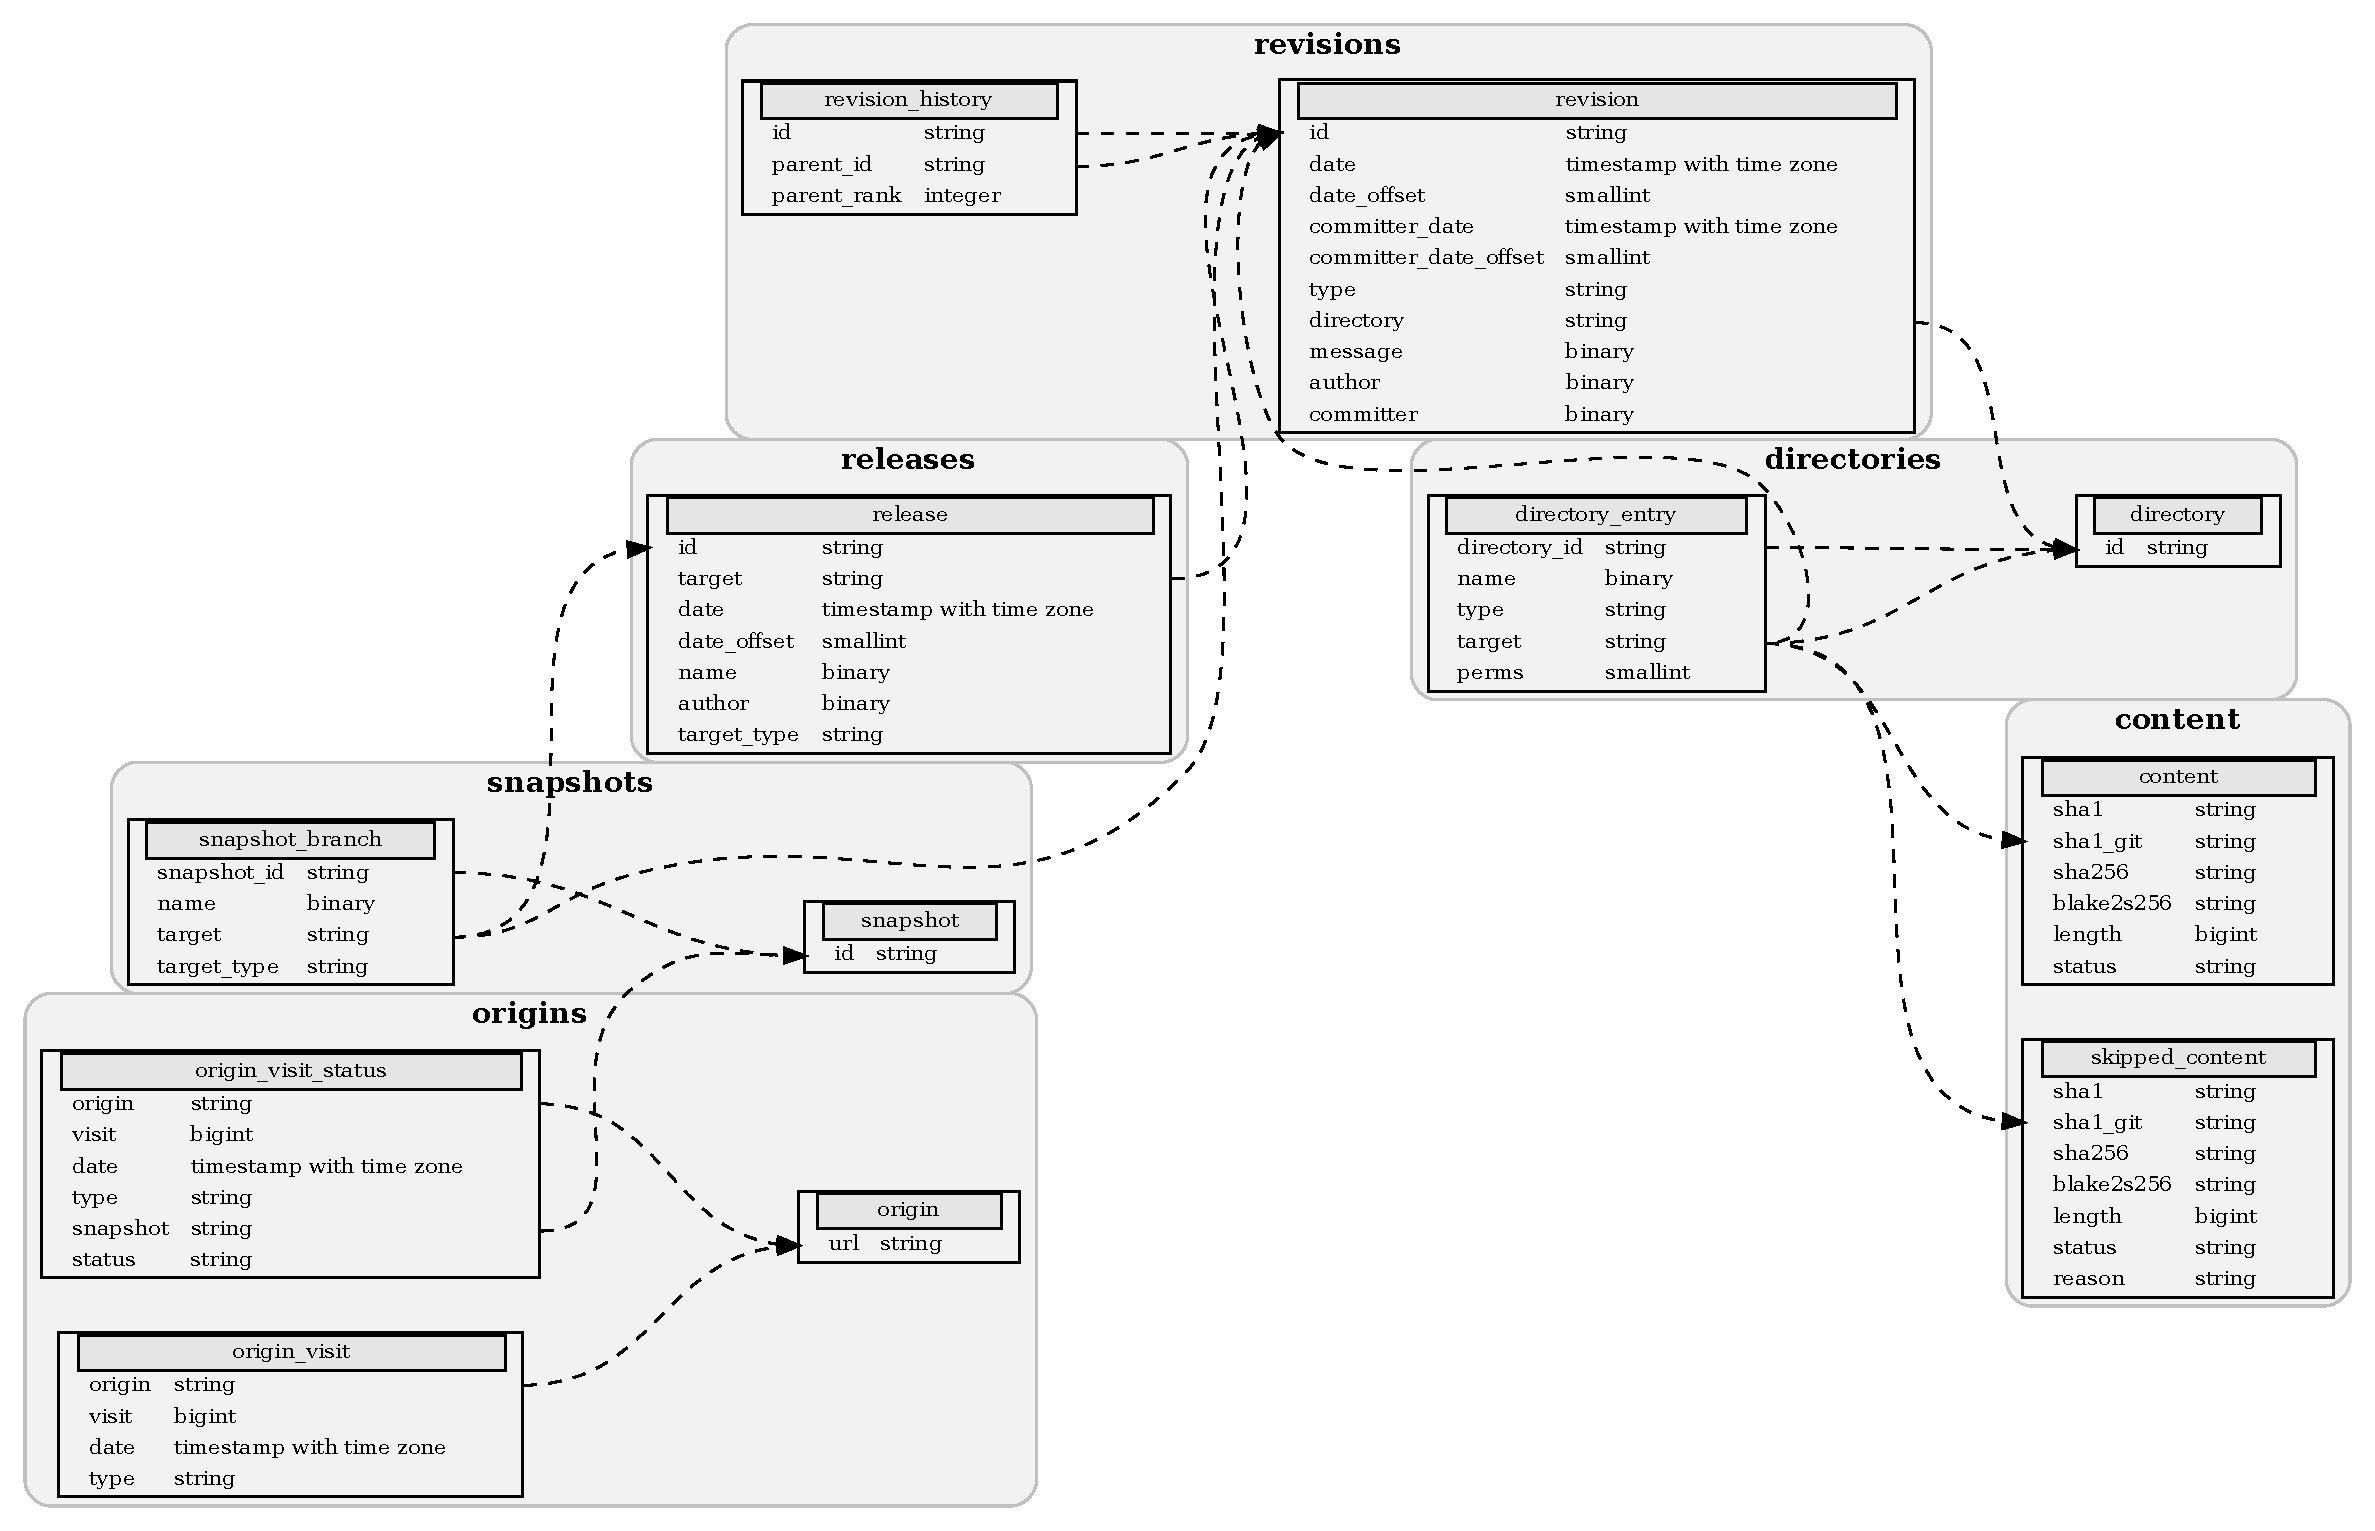
\includegraphics[height=0.3\textheight]{../img/graph-dataset/db-schema}
    \end{subfigure}%
    \begin{subfigure}{0.17\textwidth}
      {\scriptsize
        \begin{tabular}{l r}
            \hline\textbf{Table} & \textbf{\# of objects} \\ \hline
            % TODO: update figures if we make a new version of the dataset
            origin    & \num{85143957}   \\
            snapshot  & \num{57144153}   \\
            revision  & \num{1125083793} \\
            directory & \num{4422303776} \\
            content   & \num{5082263206} \\ \hline
        \end{tabular}}
        \vspace{4.1cm}
    \end{subfigure}
    \caption{Simplified schema of the \SWHGD and the number of artifacts in it}\label{fig:db-schema}%
\end{figure*}

As shown in \figref{fig:data-model}, the \SWH DAG is organized in five logical
layers, which we describe from bottom to top.

\textbf{Contents} (or ``blobs'') form the graph's leaves,
and contain the raw content
of source code files, not including their filenames (which are
context-dependent and stored only as part of directory entries).
The dataset contains cryptographic checksums for all contents though,
that can be used to retrieve the actual files from any \SWH mirror using a Web
\textsc{api}\footnote{\url{https://archive.softwareheritage.org/api/}} and
cross-reference files encountered in the wild, including other datasets.

\textbf{Directories} are lists of named directory entries.
Each entry can
point to content objects (``file entries''), revisions (``revision entries''),
or other directories (``directory entries'').

\textbf{Revisions} (or ``commits'') are point-in-time captures of the entire
source tree of a development project. Each revision points to the root
directory of the project source tree, and a list of its parent revisions.

\textbf{Releases} (or ``tags'') are revisions that have been marked as noteworthy
with a specific, usually mnemonic, name (e.g., a version number). Each release
points to a revision and might include additional descriptive metadata.

\textbf{Snapshots} are point-in-time captures of the full state of a project
development repository. As revisions capture the state of a single development
line (or ``branch''), snapshots capture the state of \emph{all} branches in a
repository and allow to deduplicate unmodified forks across the archive.

% \textbf{Origins:} information on the original source where the software was
% retrieved from, most notably its URL and additional metadata.

Deduplication happens implicitly, automatically tracking byte-identical clones.
If a file or a directory is copied to another project, both projects will point
to the same node in the graph. Similarly for revisions, if a project is forked
on a different hosting platform, the past development history will be
deduplicated as the same nodes in the graph.  Likewise for snapshots, each
``fork'' that creates an identical copy of a repository on a code host, will
point to the same snapshot node.  By walking the graph bottom-up, it is hence
possible to find all \emph{occurrences} of a source code artifact in the
archive (e.g., all projects that have ever shipped a specific file content).

The Merkle \textsc{dag} is encoded in the dataset as a set of relational tables. In
addition to the nodes and edges of the graph, the dataset also contains
crawling information, as a set of triples capturing where (an origin \textsc{url}) and
when (a timestamp) a given snapshot has been encountered. A simplified view of
the corresponding database schema is shown in \figref{fig:db-schema}; the full schema
is available as part of the dataset distribution.
The sizes of the dataset's most notable tables are shown in the legend
appearing in the Figure's top right.

\begin{comment}

\begin{itemize}
    \item The \texttt{content} table contains information on the contents
        stored in the archive. Along with some metadata on the contents (like
        the \texttt{length} column) it contains its \texttt{sha1} cryptographic
        hash. The \texttt{content\_missing} table is virtually identical, but
        for contents that were not archived for various reasons.

    \item The \texttt{directory} table contains the directories in the archive.
        Its \texttt{id} column is its intrinsic identifier, computed with the
        \texttt{sha1\_git} hashing algorithm. It contains three columns for its
        children in the graph, \texttt{dir\_entries}, \texttt{file\_entries}
        and \texttt{rev\_entries}. Each of these columns is an array of
        integers, referencing an entry in their respective tables
        \texttt{directory\_entry\_dir}, \texttt{directory\_entry\_file} and
        \texttt{directory\_entry\_rev}. These three tables have the same
        schema: the \texttt{id} integer column referenced in the arrays of the
        \texttt{directory} table, the \texttt{name} of the object (the basename
        of its path), its permissions \texttt{perms}, and the \texttt{target}
        field which references the intrinsic identifier of the node they are
        pointing towards (respectively, the \texttt{id} field of directories,
        the \texttt{sha1\_git} field of contents and the \texttt{id} field of
        revisions).

    \item The \texttt{revision} table contains all the revisions, identified by
        their intrinsic hash in the \texttt{id} field. Each revision points to
        the root directory of the project source tree, identified by the
        \texttt{directory} field which references the \texttt{sha1\_git}
        cryptographic hash of the directory.
        The table also contains metadata on the revisions, notably the
        \texttt{author} and \texttt{committer} fields, the
        \texttt{date} and \texttt{committer\_date} fields and the
        \texttt{message} field.

        Each revision has an ordered set of parents (0 for the initial commit
        of a repository, 1 for a normal commit and 2 or more for a merge
        commit). These parents are stored in the \texttt{revision\_history}
        table, one row per parent. Each parent is identified by the \texttt{id}
        identifier, pointing to the hash of the revision, the
        \texttt{parent\_id} identifier, pointing to the hash of the parent
        revision, and the \texttt{parent\_rank} integer which defines the order
        of the parents of each revision.

    \item The \texttt{person} table deduplicates commit authors by their name
        and e-mail addresses. For pseudonymization purposes and in order to
        prevent abuse, these columns were removed from the dataset, and this
        table only contains the \texttt{id} column referenced by the
        \texttt{author} and \texttt{committer} fields of the \texttt{revision}
        table. Individual authors may be retrieved using this ID from the
        Software Heritage \textsc{api}.

    \item The \texttt{release} table contains the releases in the archive. They
        are also identified by their intrinsic hash \texttt{id} and point to a
        revision referenced by its hash in the \texttt{target} field. The
        metadata fields are semantically similar to the \texttt{revision} table
        (i.e \texttt{author}, \texttt{date}, \texttt{message}).

    \item The \texttt{snapshot} table contains the list of snapshots identified
        by their intrinsic hash \texttt{id}, and their integer primary key in
        the archive \texttt{object\_id}.
        Each snapshot maps to a list of branches listed in the table
        \texttt{snapshot\_branch} through the many-to-many relationship
        intermediate table \texttt{snapshot\_branches}, which references the
        \texttt{object\_id} fields of the \texttt{snapshot} and
        \texttt{snapshot\_branch} tables. The \texttt{snapshot\_branch} table
        also contains the \texttt{name} of the branch and the \texttt{target}
        it points to (identified by its intrinsic hash), either a
        \texttt{release}, \texttt{revision}, \texttt{directory} or
        \texttt{content} object depending on the value of the
        \texttt{target\_type} field.

    \item The \texttt{origin} table contains the origins from which the
        software projects in the dataset were archived, identified by their
        \texttt{id} identifier, and \texttt{type} and \texttt{url} metadata.

        Since Software Heritage archives software continuously, software
        origins are crawled more than once. Every ``visit'' of an origin is
        stored in the \texttt{origin\_visit} table, which contains the
        identifier \texttt{origin} of the origin visited, the \texttt{date} of
        the visit and a \texttt{snapshot\_id} integer which points to the
        \texttt{object\_id} identifier of the \texttt{snapshot} table.
\end{itemize}

\end{comment}


\section{Sample Queries and Research Questions}
\label{sec:usage}
To further illustrate the dataset's affordances and as
motivating examples regarding the research possibilities
it opens,
below are some sample SQL queries that can be executed
with the dataset on \textsc{AWS} Athena.

\begin{listing}[H]
    \inputminted[firstline=4]{sql}{codesamples/graph-dataset/popular-file.sql}
    \caption{Most frequent file name}%
    \label{lst:popular-file}
\end{listing}

Listing~\ref{lst:popular-file} shows a simple query
that finds the most frequent file name across all the revisions.
The result, obtained by scanning
151~GiB\ in $3'40''$, is \texttt{index.html}, which occurs in the dataset 182
million times.

\lstinputlisting[firstline=3,float,
caption={Most common commit operations},
label=lst:popular-commit-words]{codesamples/graph-dataset/popular-commit-words.sql}

As an example of a query useful in software evolution research,
consider the Listing~\ref{lst:popular-commit-words}.
It is based on the convention dictating that commit messages should
start with a summary expressed in the imperative mood~\cite[3.3.2.1]{Fre19}.
Based on that idea, the query uses a regular expression to extract the first
word of each commit message and then tallies words by frequency.
By scanning 37~GiB\ in $30''$ it gives us that commits
concern the following common actions ordered by descending order of frequency:
\emph{add, fix, update, remove, merge, initial, create}.
(We had to manually stem some verbs,
because the most recent version of the Presto query engine,
which provides a built-in stemming function,
is not yet available on Athena.)

\lstinputlisting[firstline=3,float,
caption={Ratio of commits performed during each year's weekends},
label=lst:weekend-work]{codesamples/graph-dataset/weekend-work.sql}

SQL queries can also be used to express more complex tasks.
Consider the research hypothesis that weekend work on open source projects
is decreasing over the years as evermore
development work is done by companies rather than volunteers.
The corresponding data can be obtained by finding the ratio
between revisions committed on the weekends of each year and
the total number of that year's revisions (see Listing~\ref{lst:weekend-work}).
The results, obtained by scanning 14~GiB\ in $7''$ are inconclusive,
and point to the need for further analysis,
which is left as an exercise to the reader.

\lstinputlisting[firstline=4,float,
caption={Average number of a revision's parents},
label=lst:fork-size]{codesamples/graph-dataset/fork-size.sql}

The provided dataset forms a graph, which can be difficult query with SQL.
Therefore, questions associated with the graph's characteristics,
such as closeness, distance, and centrality, will require the use of
other query mechanisms.
Yet, interesting metrics can be readily obtained by limiting scans
to specific cases, such as merge commits.
As an example, Listing~\ref{lst:fork-size} calculates the average
number of parents of each revision ($1.088$, after scanning 23~GiB\ in $22''$)
by grouping revisions by their parent identifier.
Such queries can be used to examine in depth the characteristics
of merge operations.

\lstinputlisting[firstline=4,float,
caption={Average size of the most popular file types},
label=lst:file-type-size]{codesamples/graph-dataset/file-type-size.sql}

Although the performance of Athena can be impressive,
there are cases where the available memory resources will be exhausted
causing an expensive query to fail.
This typically happens when joining two equally large tables consisting
of hundreds of millions of records.
This restriction can be overcome by sampling the corresponding tables.
Listing~\ref{lst:file-type-size} demonstrates such a case.
The objective here is to determine the modularity at the level of files among
diverse programming languages, by examining the size of popular file types.
The query joins two 5~billion row tables:
the file names and the content metadata.
To reduce the number of joined rows a 1\% sample of the rows is processed,
thus scanning 317~GiB\ in $1'20''$.
The order of the resulting language files
(JavaScript$>$C$>$C++$>$Python$>$\textsc{php}$>$C\#$>$ Ruby)
indicates that,
with the exception of JavaScript,
languages offering more abstraction facilities are associated with
smaller source code files.


\section{Limitations and Extensions}
\label{sec:threats}

As discussed in Section~\ref{sec:gathering}, the dataset is not fully
reproducible. This is a limitation, but one that is very hard to avoid for
datasets originating from long-term archival.

The dataset cannot claim full coverage of the entire software commons, and
several forges and package repositories are still missing from it. Still, it is
the largest dataset of its kind (by several order of magnitude). Also, to
mitigate this limitation we plan to periodically publish new versions of it, as
the \SWH archive extends its coverage.

As a first future extension we plan to include actual file contents as part of
the dataset. This is currently impractical due to the storage size (\TODO{size}),
but we are exploring cloud storage with bring-your-own-compute service model
solutions.

As further extensions, it would be useful to combine the \SWHGD with neighboring
datasets that contain non-source-code development artifacts, such as issues,
code review discussions, wiki pages, etc. We are exploring an integrated
dataset with GHTorrent~\cite{DBLP:conf/msr/GousiosS12}, even thought that would
narrow the scope to GitHub ``only''.


\section{Related Work}
\label{sec:related}

% \SWH~\cite{cacm-2018-software-heritage, ipres-2017-software-heritage} is the
% archival project used as a basis for producing this dataset.

To the best of the authors' knowledge no existing dataset contains a comparable
amount of data about source code artifacts extracted from public
software development.

GHTorrent~\cite{DBLP:conf/msr/GousiosS12} covers GitHub and includes
non-source-code artifacts (e.g., issues, pull requests, etc.), but lacks other
software distribution places (e.g., GitLab, Debian, PyPI). Also, no
deduplication applies to GHTorrent, making cloning tracking more challenging.
CodeFeedr~\cite{DBLP:conf/icse/VargasHKBG18} is a natural evolution of
GHTorrent, but it is oriented toward expanding coverage for additional sources
of non-source-code artifacts.

The Debsources dataset~\cite{debsources-ese-2016} contains a wealth of
information about Debian releases over several decades, but stops at the
release granularity (rather than commits) and is at least three orders of magnitude
smaller than the present dataset.
